% @Author: Athul Vijayan
% @Date:   2014-05-09 13:56:20
% @Last Modified by:   Athul
% @Last Modified time: 2015-09-22 16:53:20

\documentclass[11pt]{article}
\usepackage[utf8]{inputenc}
\usepackage[a4paper, margin=1in]{geometry}
\usepackage{amsmath}
\usepackage[table]{xcolor}
\usepackage{amssymb}
\usepackage{graphicx}
\usepackage[toc,page]{appendix}
\usepackage{color}
\usepackage{subcaption}
\usepackage[section]{placeins}
\usepackage{rotating}
\usepackage{wrapfig}
\usepackage{bm}
\usepackage[normalem]{ulem}
\usepackage[table]{xcolor}
\newcommand{\HRule}{\rule{\linewidth}{0.2mm}} % Defines a new command for the horizontal lines, change thickness here
\usepackage{hyperref}
\hypersetup{
    colorlinks,
    citecolor=black,
    filecolor=black,
    linkcolor=black,
    urlcolor=cyan
}
\usepackage{array}
\renewcommand{\P}{\mathbb{P}}
\newcolumntype{L}[1]{>{\raggedright\let\newline\\\arraybackslash\hspace{0pt}}m{#1}}
\newcolumntype{C}[1]{>{\centering\let\newline\\\arraybackslash\hspace{0pt}}m{#1}}
\newcolumntype{R}[1]{>{\raggedleft\let\newline\\\arraybackslash\hspace{0pt}}m{#1}}
\newcommand{\rulesep}{\unskip\ \vrule\ }

%----------------------------------------------------------------------------------------
%   TITLE PAGE
%----------------------------------------------------------------------------------------

\newcommand*{\titleGM}{\begingroup % Create the command for including the title page in the document
\hbox{ % Horizontal box
\hspace*{0.2\textwidth} % Whitespace to the left of the title page
\rule{1pt}{\textheight} % Vertical line
\hspace*{0.05\textwidth} % Whitespace between the vertical line and title page text
\parbox[b]{0.75\textwidth}{ % Paragraph box which restricts text to less than the width of the page

{\noindent\Huge\bfseries  Neural data analysis}\\[2\baselineskip] % Title
{\large \textit{Notes}}\\[4\baselineskip] % Tagline or further description
{\Large \textsc{Athul Vijayan \hspace{5pt} ed11b004}} % Author name

\vspace{0.5\textheight} % Whitespace between the title block and the publisher
}}
\endgroup}


\begin{document}
% \titleGM % This command includes the title page
\tableofcontents

% =========================== content =========================
\newpage
\section{Introduction} % (fold)
\label{sec:introduction}
\subsection{Background} % (fold)
\label{sub:background}

% subsection background (end)
\subsection{Experiment} % (fold)
\label{sub:experiment}
Virus expressing GCaMP6f was injected into the V1 of mice. Approximately 3 weeks post infection, mice were imaged under a 2-photon microscope while sinusoidal drifting gratings were presented on a computer screen placed 3 inches from the mouse (1 degree of visual space $\sim$ 21.3 pixels on the screen). The stimulus was varied as:
\begin{enumerate}
    \item Sinusoidal drifting gratings at 16 different directions (0:22.5:337.5). Spatial frequency was fixed at 0.03 cycles per degree.
    \item Each direction was repeated 10 times (i.e. 10 trials per direction). Directions are presented in a randomized order.
    \item Each direction was presented for 2s and was always preceded by a 4s gray screen. Therefore the total duration of the stimulus is 6s.
    \item Calcium signals (GCaMP6f in awake mice) were acquired from awake mice at 20 frames per seconds. Thus, sampling rate is 20Hz.
\end{enumerate}
 
% subsection experiment (end)

\subsection{Aim} % (fold)
\label{sub:aim}
\begin{itemize}
    \item To map orientation tuning responses of excitatory pyramidal neurons in V1.
    \item To determine response reliability at preferred orientation.
    \item To determine signal and noise correlations between neuron as a function of orientation tuning.
\end{itemize}
% subsection aim (end)

\section{Dataset} % (fold)
\label{sec:dataset}

\textbf{Notes about Data.mat}\\
Data.mat contains 4 entries:
\begin{enumerate}
    \item Data.rawF =  raw fluorescence values. Matrix size = number of cells x number of frames.
    \item Data.dFF    = fluorescence normalized to baseline (dFF =  (F-F0)/F0, where F0 is the baseline fluorescence computed using a sliding window of 400 frames). Same size as above.
    \item Data.Spks  = inferred spike rate using the Vogelstein deconvolution algorithm. Same size as above.
    \item Data.StimSeq = contains sequence of directions presented during that experiment. Vector size = 160 x 1.
\end{enumerate}
\textbf{Notes about Ori.mat}\\
Ori.mat contains 20 entries. The most pertinent entries are:
\begin{enumerate}
    \item Ori.OSI = orientation selectivity indices of the neurons
    \item Ori.OrFit = double-wrapped Gaussian fits
    \item Ori.OrFitQuality  = goodness of Gaussian fits. (Higher the percentage value, the better the fit)
    \item Ori.Width = tuning width in degrees
    \item Ori.PrefOri = preferred orientation
    \item Ori.SpkResponse = Contains neural responses for each cells sorted according to the different directions. Size: 1xNumber of cell Cell array. Each cell entry contains a 1x Number of Direction Cell array, which contains a Number of Frames x Trials matrix.
\end{enumerate}

\subsection{Restructuring the data} % (fold)
\label{sub:restructuring_the_data}
There are 19200 Ca readings for each mouse. The experiment is done using 16 different stimuli, Let us think of it as 16 classes. The angle of the drifting pattern changes between the classes. It is implicit that $0^{o}$ and $180^{o}$ will have same orientation, but the direction of drifting will be opposite.\\
First, the data is split into 16 parts corresponding to each class. There are 10 trials for each class. The data is split into 160 subsequences of $19200/160 = 120$ length. Now this is a time-series of 120 points for each trial, and there are ten sets of data for each class.\\
120 points in the data represents 6 seconds of brain activity. Out of the 6 seconds, first 4 seconds (80 samples for sampling frequency of 20Hz) correspond to no-stimuli (or Gray stimuli). This represents the background activity of the neuron. The last 40 samples show the response for the intended stimuli.
\begin{itemize}
    \item cellData{i} contains all data for neuron i
    \item cellData{i} is a 160$\times$121 matrix.
    \item Each row represents a single experiment. and corresponding gray duration.
    \item In a row first 120 entries show the time series data of 6 seconds (120 samples) long trial. First 4s (80 samples) gray time and last 2s (40 samples) stimuli time.
    \item Last column contain the angle of visual stimuli in radians. (class)
\end{itemize}

% subsection restructuring_the_data (end)

\section{Analysis} % (fold)
\label{sec:analysis}
Analysis is broken down into various problem statements. Various methods are considered for each of the problem statements.
\subsection{Quantifying the neuron activity} % (fold)
\label{sub:quantifying_the_neuron_activity}
The 120 point time series provide the activity of single cell in response to a particular stimulus in a trial. The activity of cell has to be studied. The first 80 samples are expected to have spikes due to only background activity, as the stimulus was gray during that time. Peaks in Ca concentration denotes the spikes in the neuron. From neuroanatomy, spike rate is a good quantify to measure neuron activity. In Calcium imaging, the amplitudes corresponds to Ca ion concentration. From the neuron models, more the Ca concentration, more is the spike rate. Following methods are used for quantifying spike rate.\\
Using various methods, a time sequence $F_t$ is calculated. $F_t$ represents the spiking activity of neuron. A relatively large $F_t$ represents a spike and small corresponds to no-spike. Number of spikes in an interval is what we seek. In the 120 sample data, $F_t$ of size 120 is found using various methods. Finally, spike rate is calculated by subtracting the background activity from the response.
$$spikeRate = \frac{\sum_{n=81}^{120} F_n}{40} - \frac{\sum_{n=1}^{80} F_n}{80}$$
Various methods for finding $F_t$ is the first problem statement. Following approaches are made to solve this.
\subsubsection{Averaging } % (fold)
\label{ssub:averaging}
The Calcium signal amplitudes averaged and the average is believed to be a proxy for the spike rate. From the smoothed data, just taking the mean of last 40 samples (time during which stimuli was presented) provides the estimated spike rate for that trial.
% subsubsection thresholding (end)

\subsubsection{Autoregressive model} % (fold)
\label{ssub:ar_model}

% subsubsection moving_average_model (end)

% subsection quantifying_the_neuron_activity (end)
\FloatBarrier
\subsection{Estimating orientation selectivity of neuron} % (fold)
\label{sub:estimating_orientation_selectivity_of_neuron}
Neurons in the striate cortex of primary visual cortex in the brain are of three types. Cells which respond to orientation of a contrasting visual stimuli and which are not sensitive to orientation. Among the orientation selective cells, some cells are also sensitive to motion of the stimuli in a particular direction in addition to orientation. These cells are called complex cells. Cells which are only sensitive  to orientation, but not to motion are called simple cells. These cells are pyramidal in structure and have a receptive field in shape of a rectangular slit. This section deals with methods to quantify the selective behavior of these cells from experimental data.

\subsubsection{Selectivity Index measures - OSI, DSI} % (fold)
\label{ssub:traditional_selectivity_measures_oi_di_and_osi}
OI and DI are used as the normalized measures of ``peak to trough'' orientation selectivity and direction selectivity.
These quantities are defined as:
\begin{align}
    OSI &= \frac{(R_{pref\_ori} - R_{orth})}{(R_{pref\_ori} + R_{orth})}\\
    DSI &= \frac{(R_{pref} - R_{null})}{(R_{pref} + R_{null})}
\end{align}
The response at the preferred orientation $R_{pref\_ori}$ and the response at the preferred direction $R_{pref}$ can be determined in different ways. In some measures, these are taken to be the best response to one of the stimulus orientations or directions that was explicitly measured; that is, if we measure responses at stimulus directions $\theta_1, \cdots, \theta_n$, then we choose the response at the best $\theta_i$ . In other measures, we perform a fit to the tuning curve, and choose the maximum value of the fit as $R_{pref\_ori}$ or $R_{pref}$ .\\
This approach is more sensitive to noise. One of the plot of spike rate vs angle of stimuli of a neuron is shown in Figure ~\ref{angle_resp}.
\begin{figure}
\centering
\caption{Comparing response of a neuron Vs angle of stimuli with the expected response}
\label{angle_resp}
\begin{subfigure}{.48\textwidth}
    \centering
    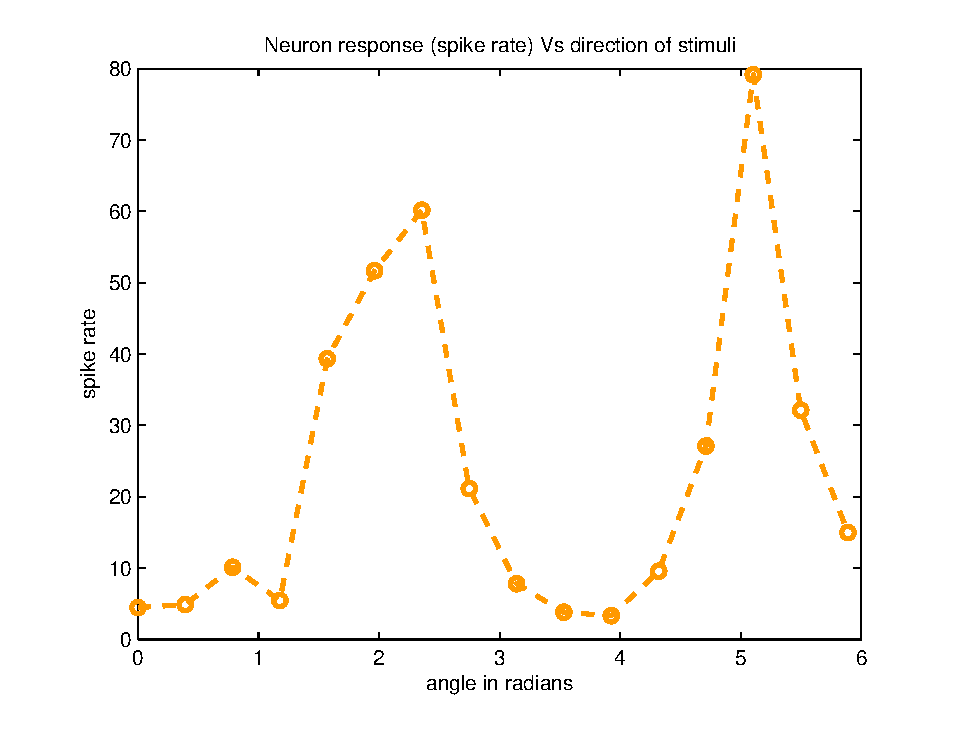
\includegraphics[width=\linewidth]{plots/max_osi}
    \caption{Spike rate vs angle of stimuli of a neuron}
\end{subfigure}
\rulesep
\begin{subfigure}{.48\textwidth}
    \centering
    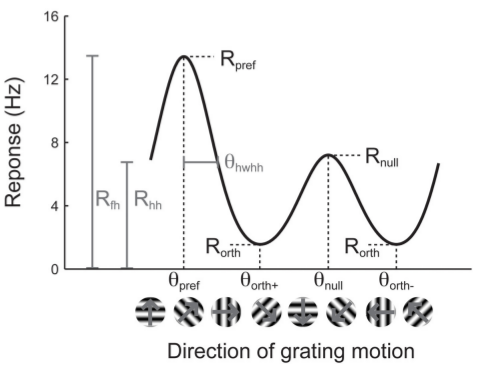
\includegraphics[width=\linewidth]{plots/typical_response.png}
    \caption{Spike rate vs angle of stimuli of a typical orientation selective neuron}
\end{subfigure}
\end{figure}
% subsubsection traditional_selectivity_measures_oi_di_and_osi (end)

\subsubsection{Circular variance of direction and orientation} % (fold)
\label{ssub:circular_variance_of_direction_and_orientation}
As discussed in the paper, Circular variance is a more robust quantifier of orientation and direction selectivity. A scalar value representing the neuron response is extracted from the 6s long time series for each of the orientations and directions (There are 8 orientations and 16 directions). As we have 10 trials for each class, we will have 160 such values for each neuron.\\
The values are first expressed as vectors in the orientation space. The vector sum of the values provide the `preferred orientation'; Magnitude should indicate how much orientation selective the neuron is.\\
Let $R(\theta)$ be the response of neuron to angle $\theta$ and we denote the `preferred direction' as $\theta_{pref}$.
Normalized vector sum in orientation and direction space is found as.
\begin{align}
    L_{ori} &= \frac{\sum_{k} R(\theta_k) exp(2\theta_k)}{\sum_{k} R(\theta_k)}\\
    L_{dir} &= \frac{\sum_{k} R(\theta_k) exp(\theta_k)}{\sum_{k} R(\theta_k)}
\end{align}
\begin{itemize}
    \item Neurons with orientation selectivity are expected to have high $L_{ori}$.
    \item Simple cells are orientation selective, but less direction selective. They are expected to have large $L_{ori}$ and small $L_{dir}$.
    \item Complex cells are orientation selective as well as direction selective. They are expected to have both large $L_{ori}$ and large $L_{dir}$.
\end{itemize}
Circular orientation variance and direction variance is given as
\begin{align}
    CirVar = 1 - |L_{ori}|\\
    DirCirVar = 1- |L_{dir}|
\end{align}
Following shows plots of orientation and direction selectivity of various kinds of neurons.
\begin{enumerate}
    \item \textbf{Orientation selective simple cell}\\
    Refer Figure~\ref{max_cirvar}
    \begin{figure}
    \centering
    \caption{Orientation selective simple cell}
    \label{max_cirvar}
    \begin{subfigure}{.48\textwidth}
        \centering
        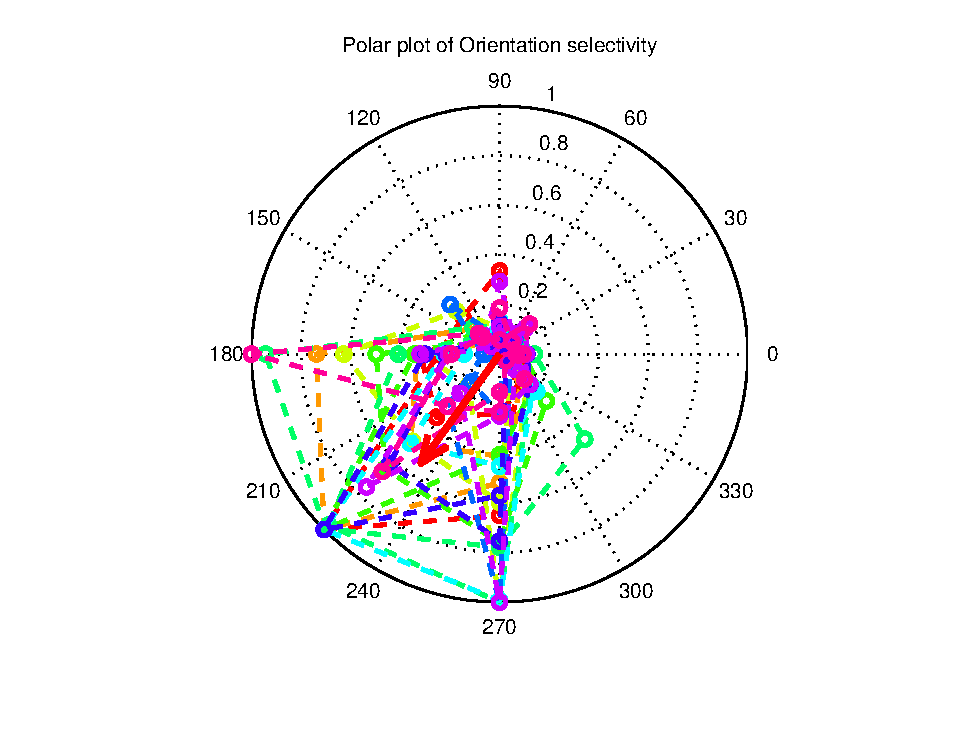
\includegraphics[width=\linewidth]{plots/max_cirvar_ori}
        \caption{Orientation selectivity plot of an orientation selective simple cell. Each curve shows a trial. Note that the cell is sensitive to an optimal orientation. The red arrow represents the direction and magnitude of orientation selectivity}
    \end{subfigure}
    \rulesep
    \begin{subfigure}{.48\textwidth}
        \centering
        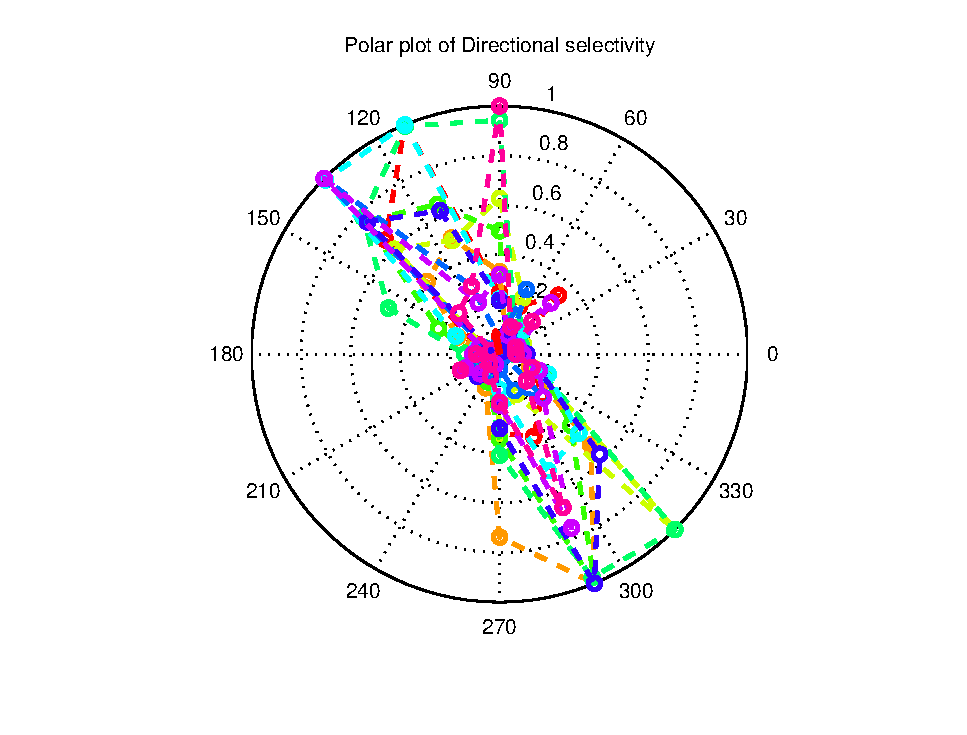
\includegraphics[width=\linewidth]{plots/max_cirvar_dir}
        \caption{Directional selectivity plot of an orientation selective simple cell. Each curve shows a trial. Note that the cell is not selective to direction, but is sensitive to orientation. The red arrow represents the direction and magnitude of direction selectivity}
    \end{subfigure}
    \end{figure}
    \item \textbf{Direction selective complex cell}\\
    Refer Figure~\ref{max_dircirvar}
    \begin{figure}
        \centering
        \caption{Direction selective complex cell}
        \label{max_dircirvar}
        \begin{subfigure}{.48\textwidth}
            \centering
            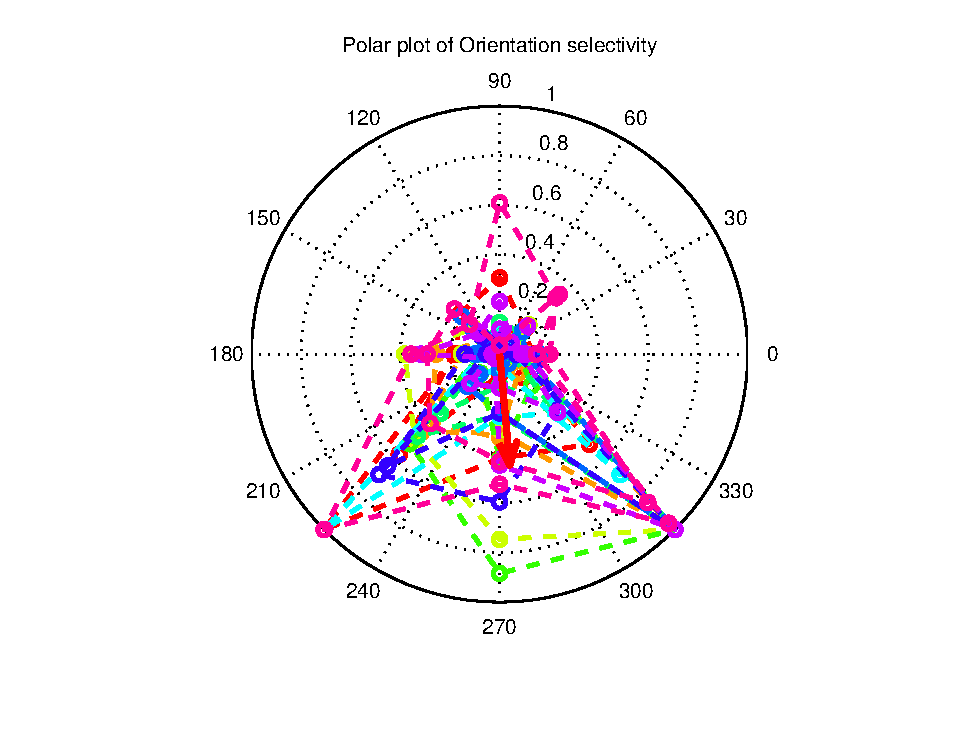
\includegraphics[width=\linewidth]{plots/max_dircirvar_ori}
            \caption{Orientation selectivity plot of an direction selective complex cell. Each curve shows a trial. Note that the cell is sensitive to an optimal orientation. The red arrow represents the direction and magnitude of orientation selectivity}
        \end{subfigure}
        \rulesep
        \begin{subfigure}{.48\textwidth}
            \centering
            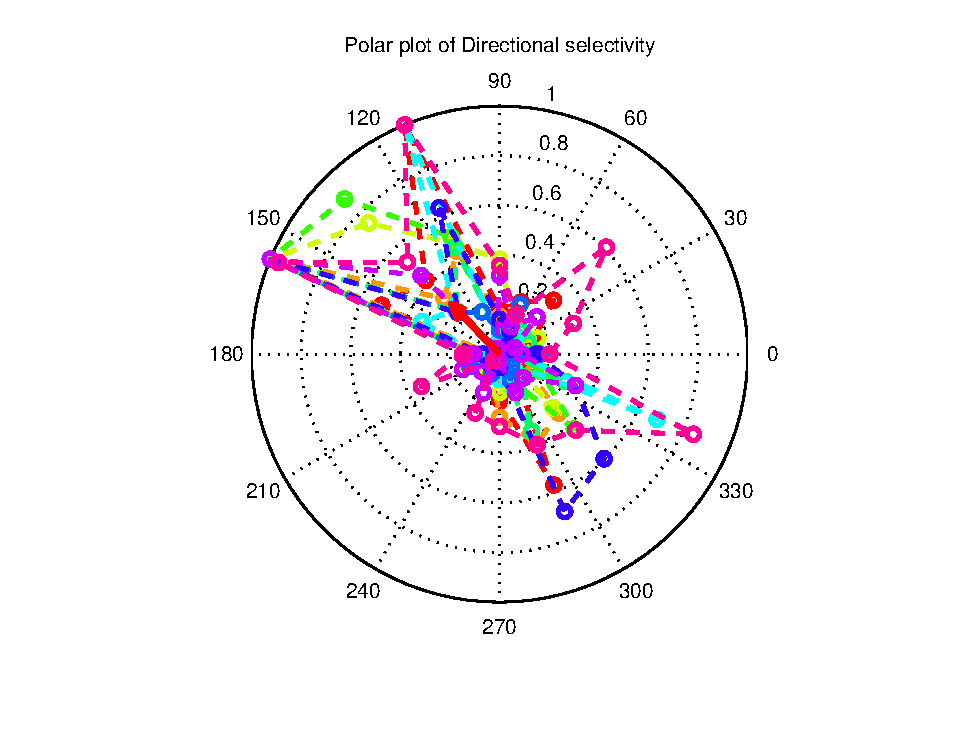
\includegraphics[width=\linewidth]{plots/max_dircirvar_dir}
            \caption{Directional selectivity plot of an direction selective complex cell. Each curve shows a trial. Note that the cell is selective to direction as well as orientation. The red arrow represents the direction and magnitude of direction selectivity}
        \end{subfigure}        
    \end{figure}
    \item \textbf{Orientation and direction Un-selective cells}\\
    Refer Figure~\ref{min_cirvar}
    \begin{figure}
        \centering
        \caption{Orientation and direction Un-selective cells}
        \label{min_cirvar}
        \begin{subfigure}{.48\textwidth}
            \centering
        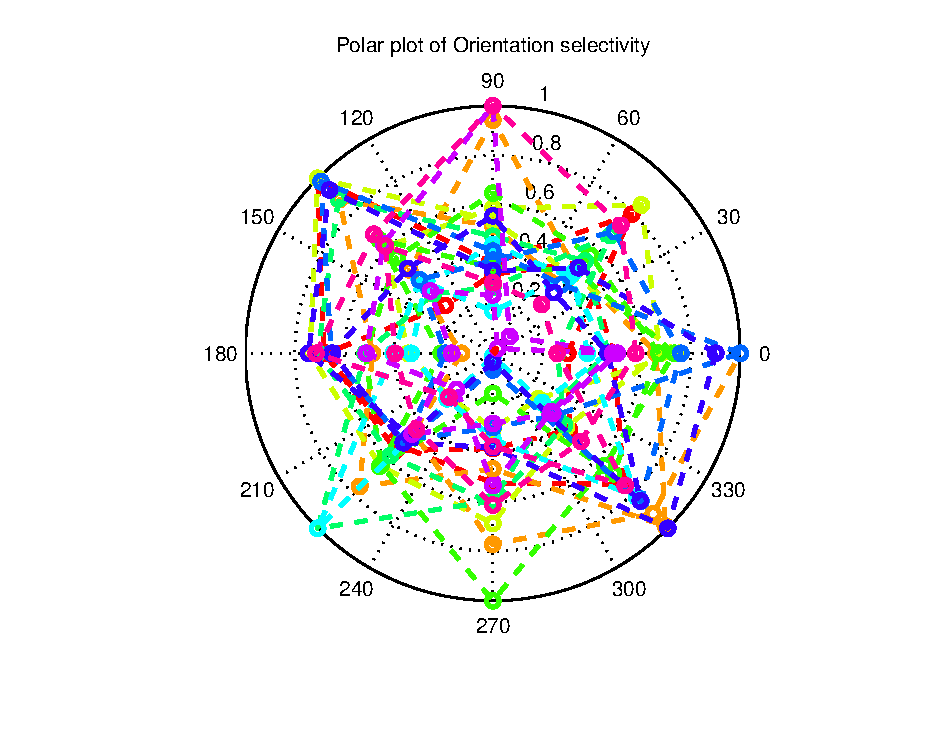
\includegraphics[width=\linewidth]{plots/min_cirvar_ori}
            \caption{Orientation selectivity plot of an Orientation and direction Un-selective cell. Each curve shows a trial. Note that the cell is uniformly sensitive to all orientations. The red arrow represents the direction and magnitude of orientation selectivity. Note the small magnitude}
        \end{subfigure}
        \rulesep
        \begin{subfigure}{.48\textwidth}
            \centering
            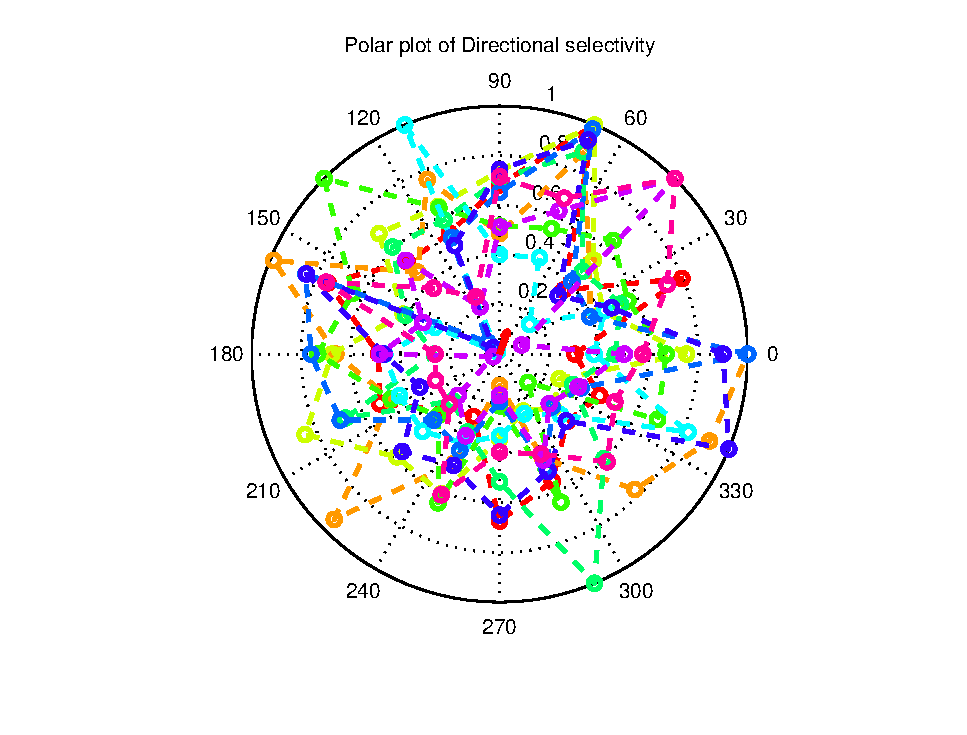
\includegraphics[width=\linewidth]{plots/min_cirvar_dir}
            \caption{Directional selectivity plot of an Orientation and direction Un-selective cell. Each curve shows a trial. Note that the cell is uniformly sensitive to all directions. The red arrow represents the direction and magnitude of direction selectivity. Note the small magnitude}
        \end{subfigure}
    \end{figure}
\end{enumerate}

\subsubsection{Measure of reliability - confidence intervals} % (fold)
\label{ssub:measure_of_reliability_confidence_intervals}

% subsubsection measure_of_reliability_confidence_intervals (end)
\FloatBarrier
\subsection{Modeling the neuron response} % (fold)
\label{sub:modeling_the_neuron_response}
Different measures of orientation selectivity are obtained from the experimental data, aim is to find metrics which represent `true' orientation selectivity. Modeling the response of neuron to various orientations and visualizing is a great way to see if in fact there is a orientation selectivity. If the cell seems selective, further inference can be drawn from models.\\
In neural data, even though fitting is a good 
From plotting the spike rate vs theta curve, We can model orientation selectivity of neuron with a Gaussian curve. We can also model the directional selectivity of a orientation/direction selective neuron using mixture of two Gaussian curves. Figure shows~\ref{gauss} a mixture of two Gaussian.\\
Some Intuitions drawn are
\begin{itemize}
    \item Fitting is `blind'. As we do not know the `true' tuning curve. Though, we can compute the error of fit to test data for judging the model.
    \item Orientation selective neurons will have distinct peaks in both, or they will have low variance parameter.
    \item Orientation unselective cells are expected to have uniform response to all angles, thus the Gaussian fit will be poor and the variance parameter will have large values.
    \item If both peaks in double Gaussian are similar, the cell is not direction specific. It has similar response to both directions, this could be a simple cell.
    \item For each neuron, the parameters will change. The `mean' parameter will decide the preferred orientation/selectivity. The variance will decide the degree to which they are selective.
    \item For fitting Gaussian,  we have 320 points. the estimation need not be accurate.
    \item For fitting double Gaussian,  we have 160 points. the estimation need not be accurate.
\end{itemize}

\begin{figure}
\centering
\caption{Modeling orientation and directional selectivity using Gaussians}
\label{gauss}
\begin{subfigure}{.48\textwidth}
    \centering
    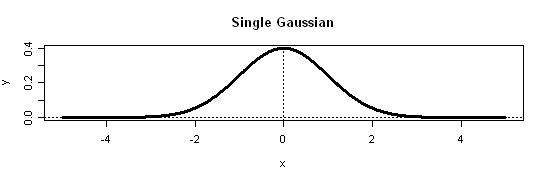
\includegraphics[width=\linewidth]{plots/gauss.png}
    \caption{Gaussian distribution}
\end{subfigure}
\rulesep
\begin{subfigure}{.48\textwidth}
    \centering
    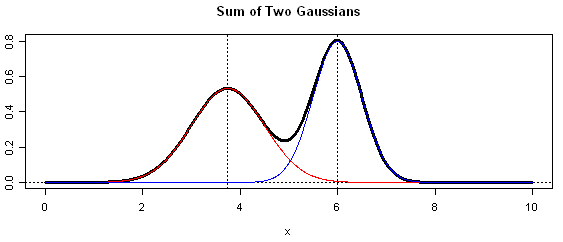
\includegraphics[width=\linewidth]{plots/double_gauss.png}
    \caption{Mixture of two Gaussians.}
\end{subfigure}
\end{figure}

\subsubsection{Estimating orientation fit} % (fold)
\label{ssub:estimating_orientation_fit}
The empirical model for orientation tuning curve is
$$R(\theta) = C + R_p \exp\{\frac{-||\theta-\theta_{pref}||^2}{2\sigma^2}\}$$
Where parameters $\theta_{pref}$ and $R_p$ are to be estimated. $\sigma$ is the tuning width, which can tell us how much the cell is selective. $C$ is a constant offset.\\
Estimation of four parameters are done my minimizing squared sum of error. Sum of squared error is defined as:
$$SSE = \sum_{i=1}^N ||R(\theta_i) - C - R_p \exp\{\frac{-||\theta_i-\theta_{pref}||^2}{2\sigma^2}\}||^2$$
The optimization is done using gradient descent algorithm.\\

% subsubsection estimating_orientation_fit (end)

\subsubsection{Estimating direction fit} % (fold)
\label{ssub:estimating_direction_fit}
The empirical model for direction tuning curve is
$$R(\theta) = C + R_p \exp\{\frac{-||\theta-\theta_{pref}||^2}{2\sigma_1^2}\} + R_n \exp\{\frac{-||\theta-\theta_{null}||^2}{2\sigma_2^2}\}$$
Where parameters $\theta_{pref}, \theta_{null}, R_n$ and $R_p$ are to be estimated. By theory, $\theta_{pref} = 180 \pm \theta_{null}$. Here $\sigma_1$ and $\sigma_2$ are the tuning widths, which can tell us how much the cell is selective. $C$ is a constant offset.
\subparagraph{Results} % (fold)
\label{subp:results}
Least squares estimation is used to find the parameters of the model. The curve fitting converged with a `good' guess of initial parameter estimate. One basis of finding direction selective cells will be to analyze the parameters of the best fit. Figure~\ref{fit_complex} shows some of the fits for complex/simple cells.
\begin{figure}
    \centering
    \begin{subfigure}{.48\textwidth}
        \centering
        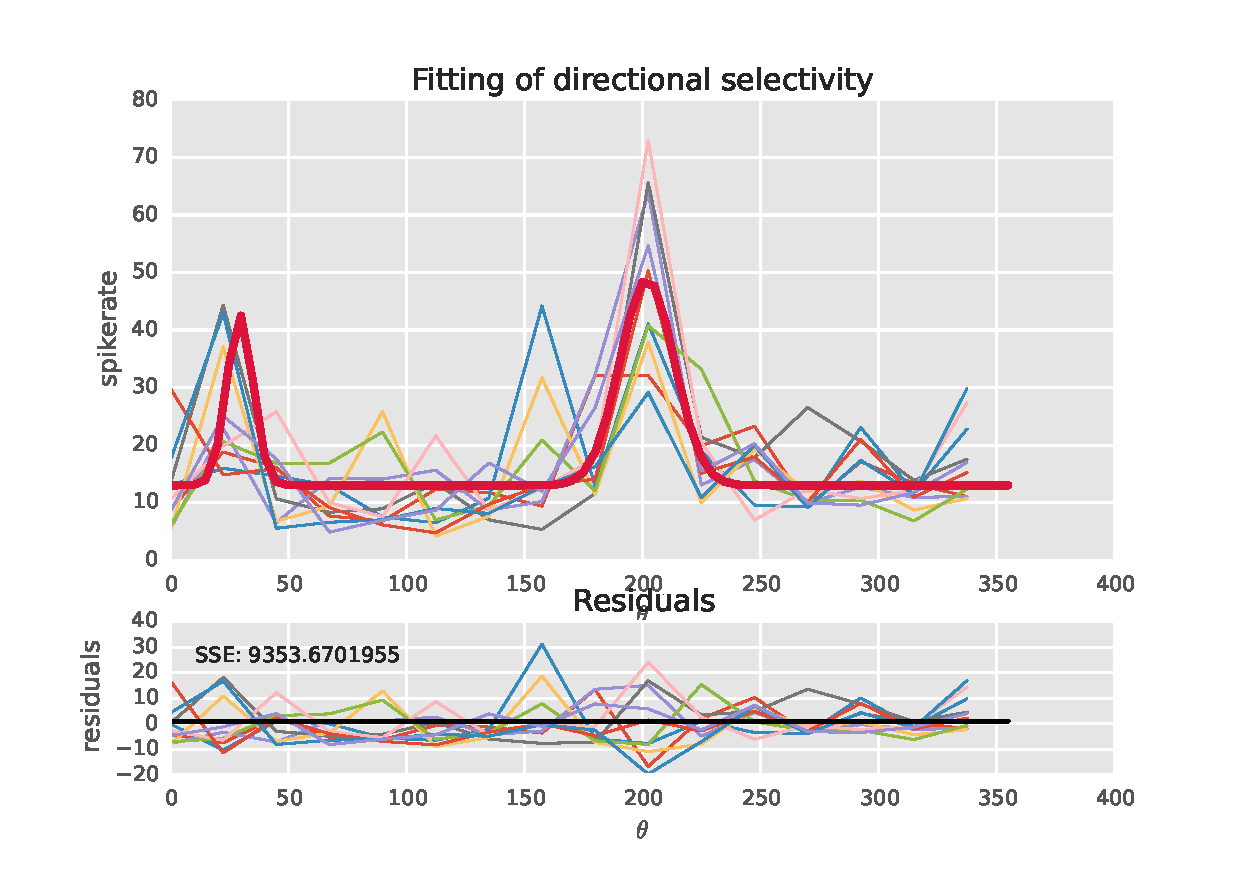
\includegraphics[width=\linewidth]{plots/fit_complex1}
    \end{subfigure}
    \begin{subfigure}{.48\textwidth}
        \centering
        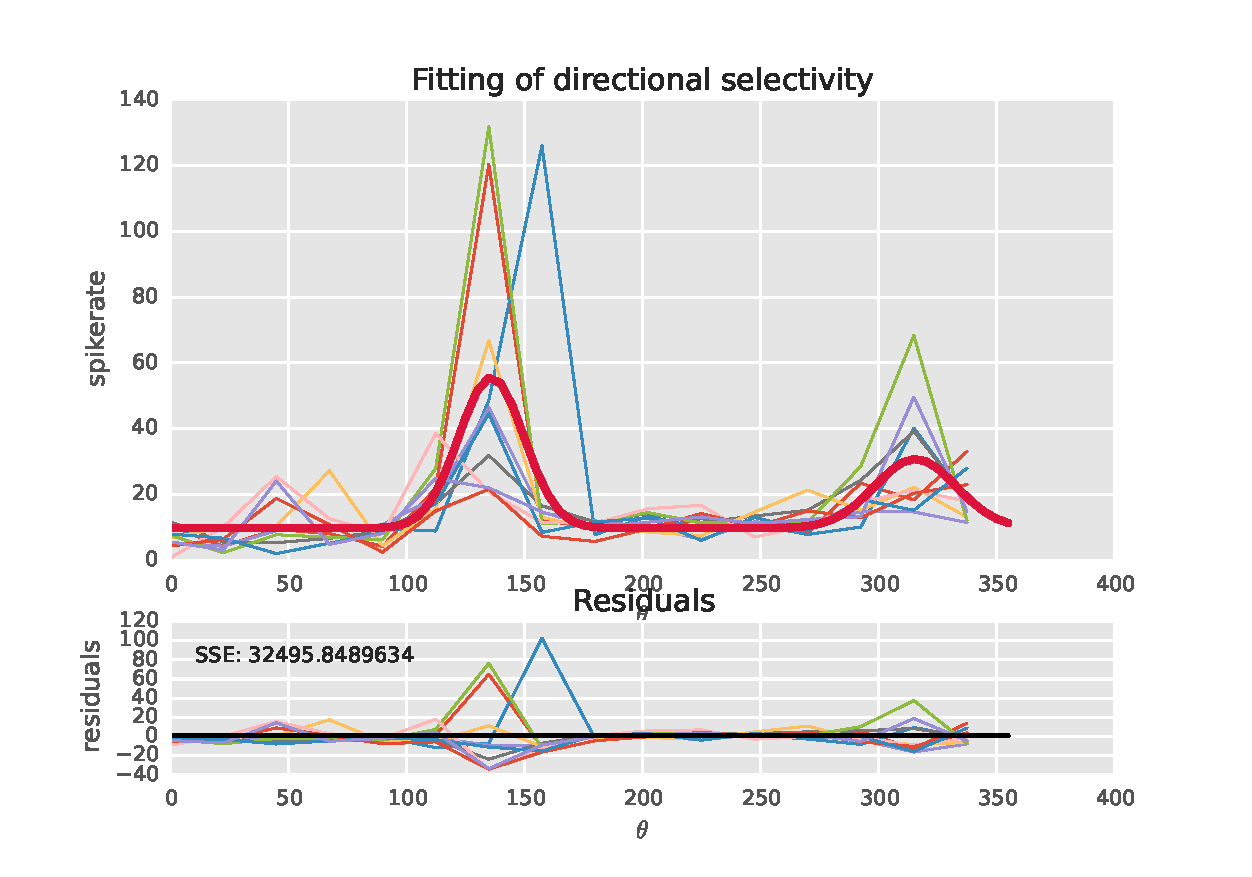
\includegraphics[width=\linewidth]{plots/fit_complex2}
    \end{subfigure}
    \newline
    \begin{subfigure}{.48\textwidth}
        \centering
        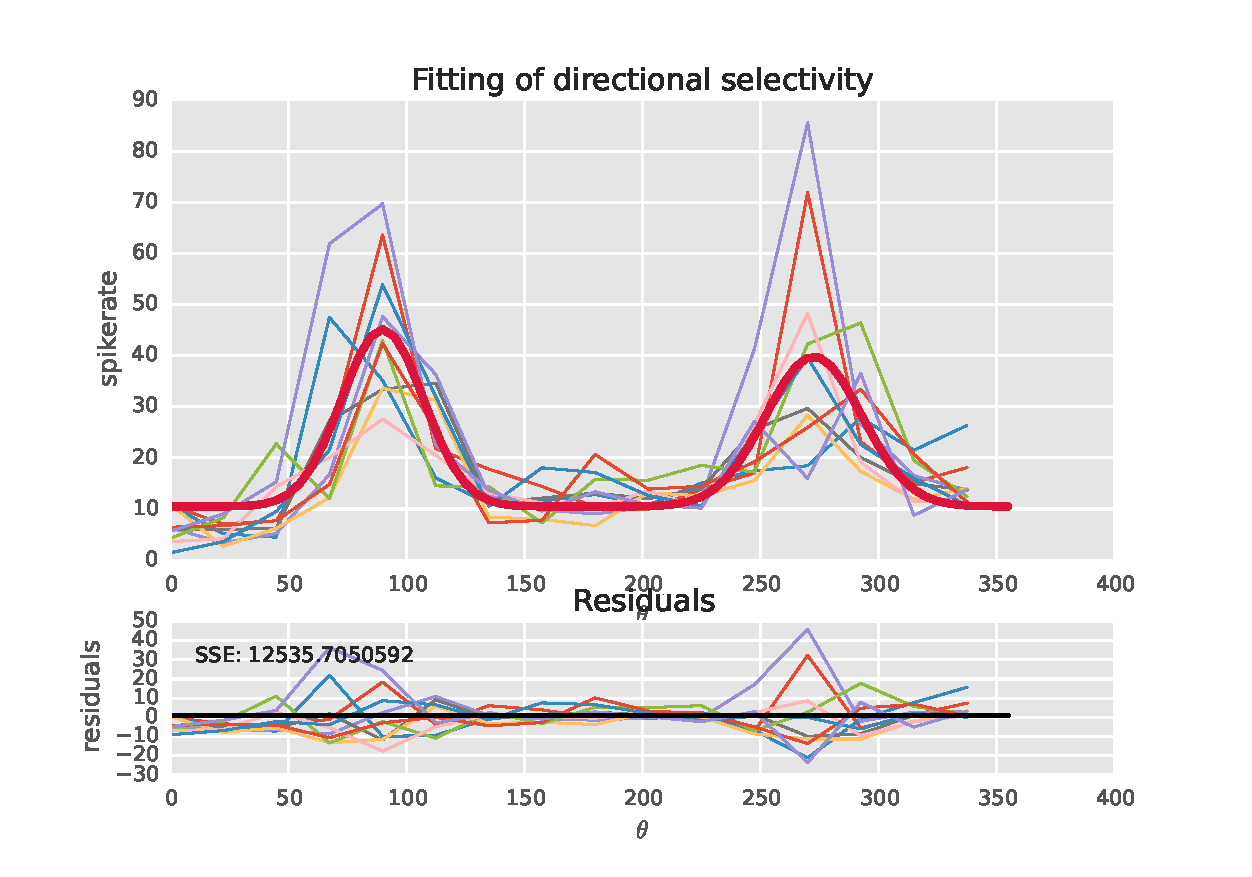
\includegraphics[width=\linewidth]{plots/fit_complex3}
    \end{subfigure}
    \begin{subfigure}{.48\textwidth}
        \centering
        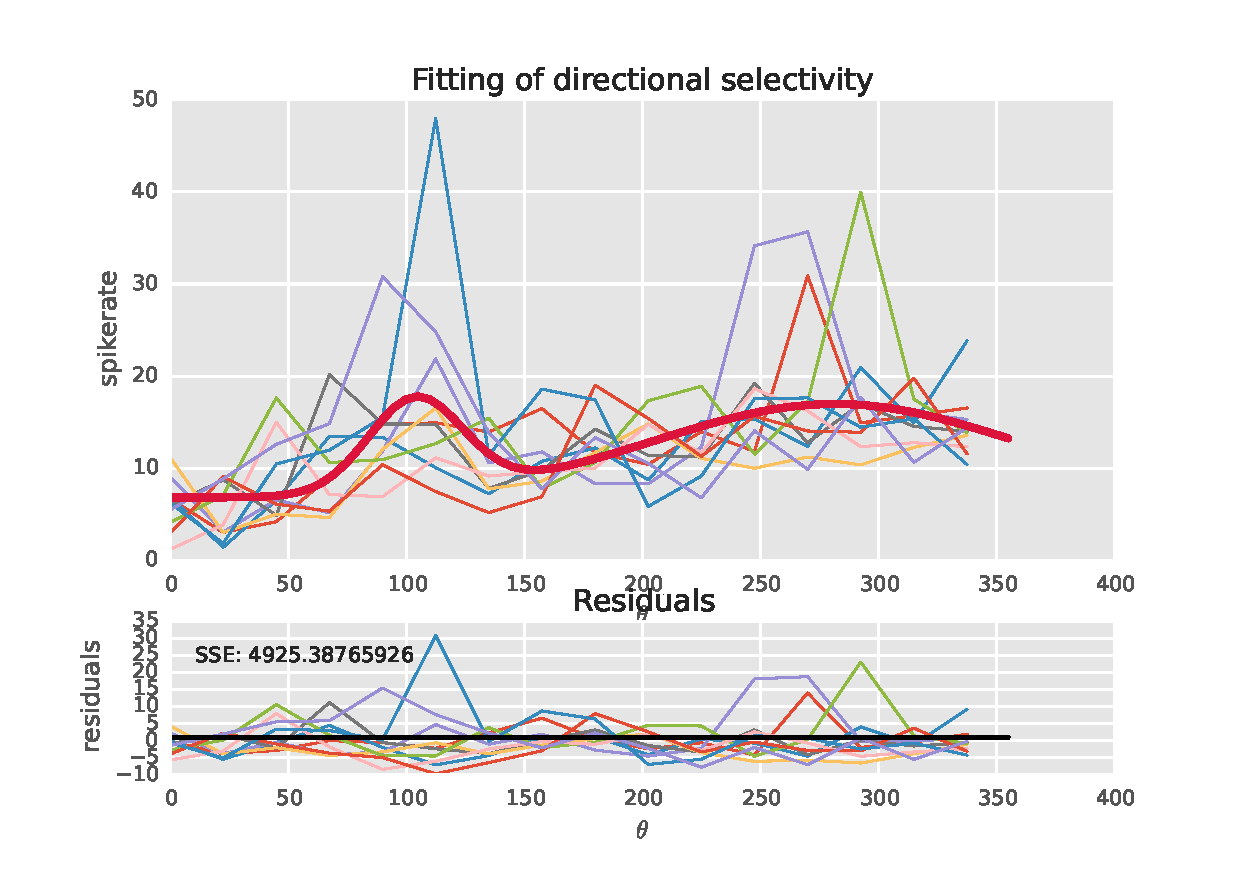
\includegraphics[width=\linewidth]{plots/fit_complex4}
    \end{subfigure}
    \caption{Fit of directional selectivity of complex cell (probably). The red curves show the fit and other curves are measured data}
    \label{fit_complex}
\end{figure}
Figure~\ref{fit_unsel} shows effort to fit the model to a direction/orientation unselective cell.
\begin{figure}
    \centering
    \begin{subfigure}{.48\textwidth}
        \centering
        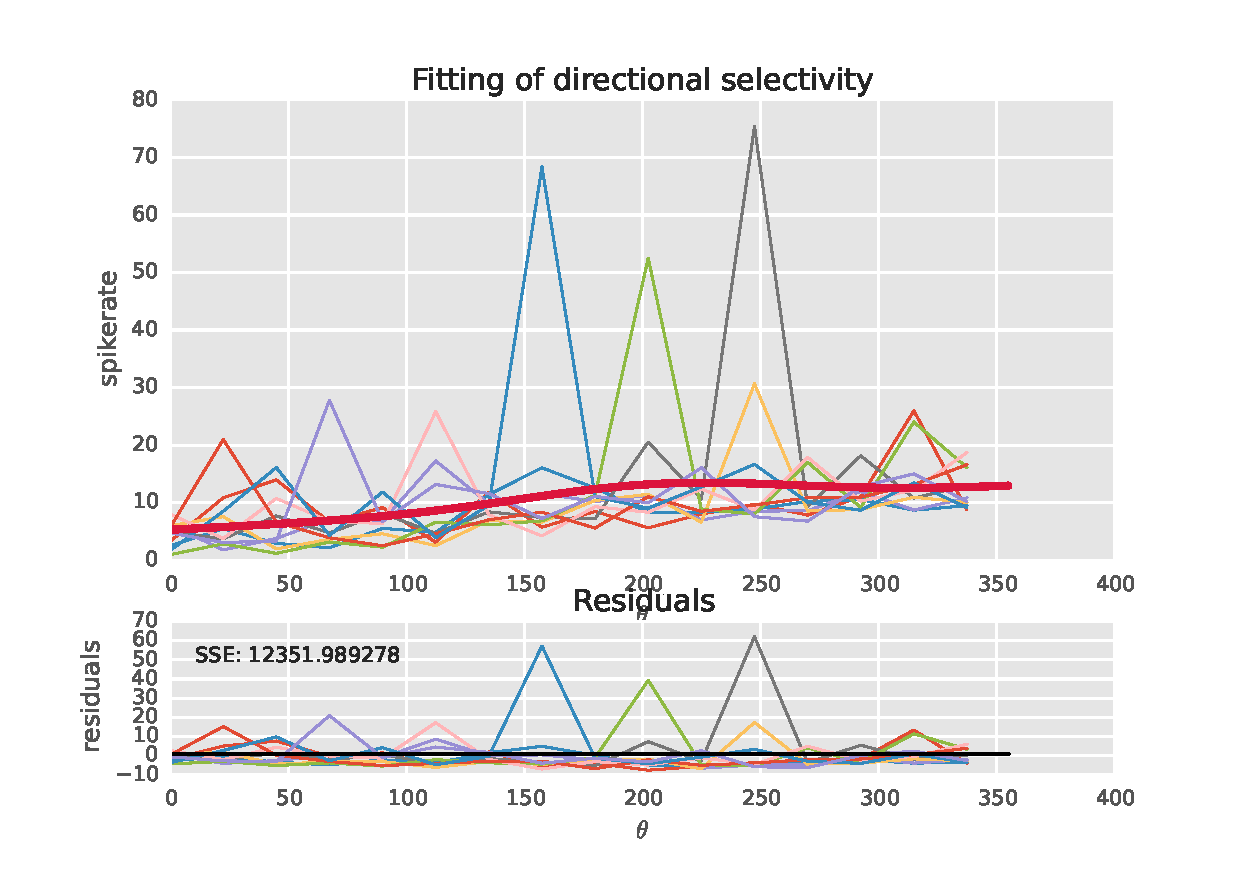
\includegraphics[width=\linewidth]{plots/fit_unsel1}
    \end{subfigure}
    \begin{subfigure}{.48\textwidth}
        \centering
        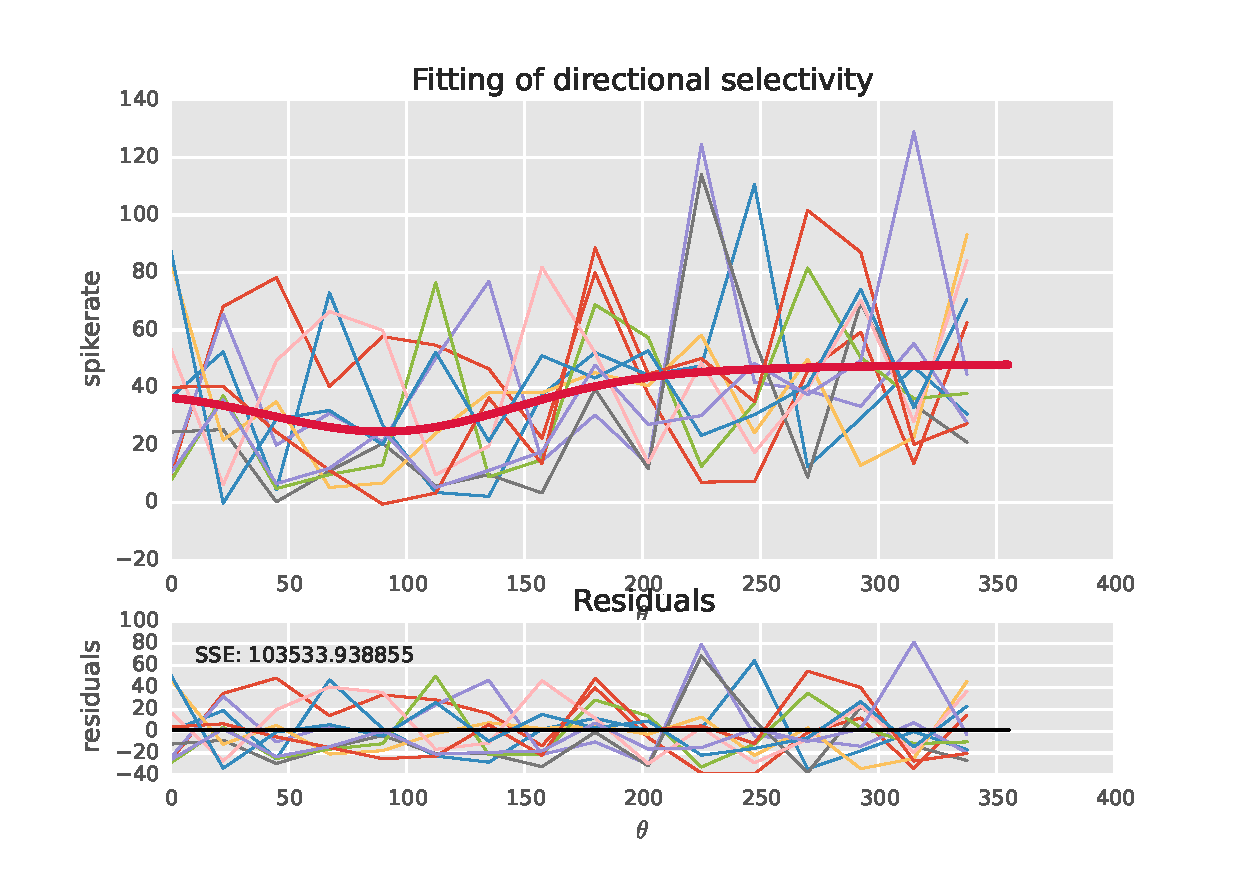
\includegraphics[width=\linewidth]{plots/fit_unsel2}
    \end{subfigure}
    \newline
    \begin{subfigure}{.48\textwidth}
        \centering
        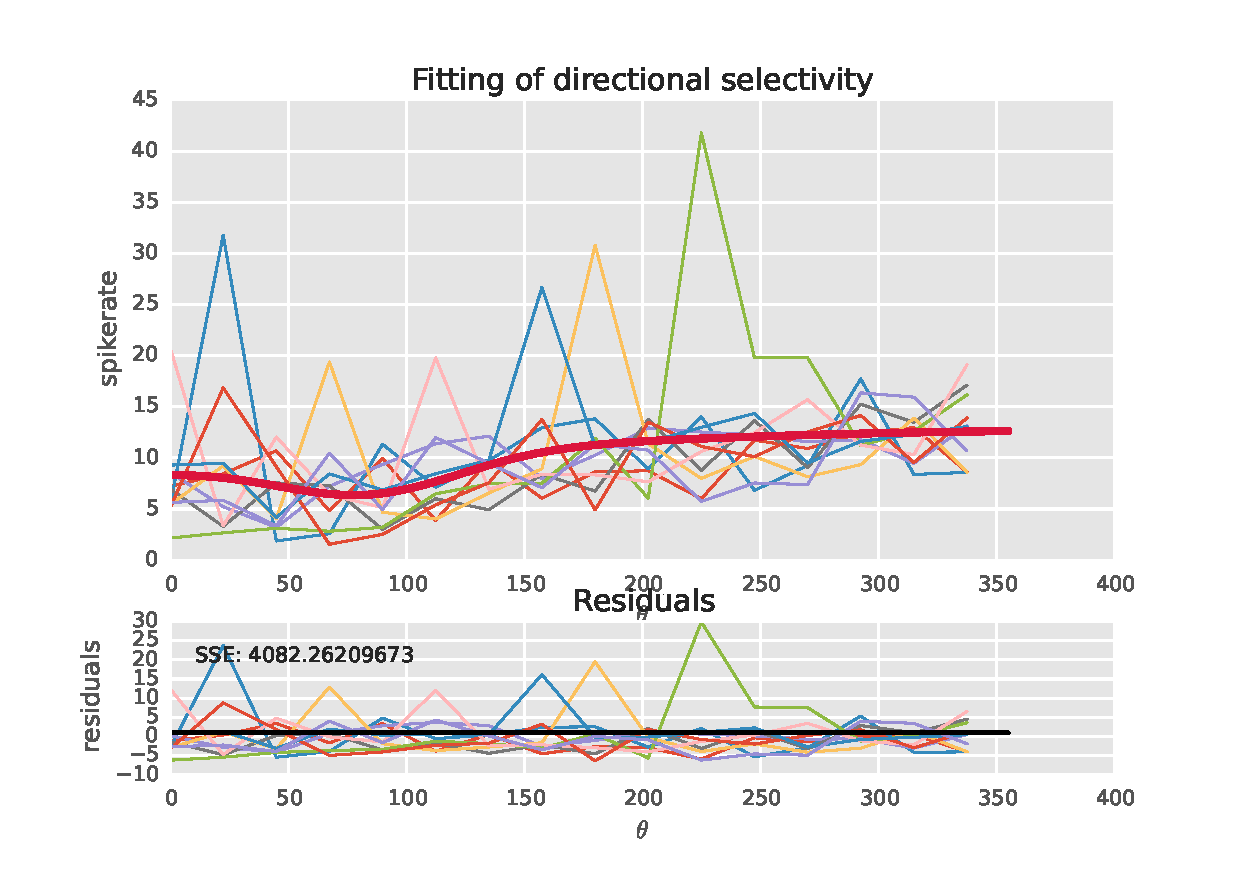
\includegraphics[width=\linewidth]{plots/fit_unsel3}
    \end{subfigure}
    \begin{subfigure}{.48\textwidth}
        \centering
        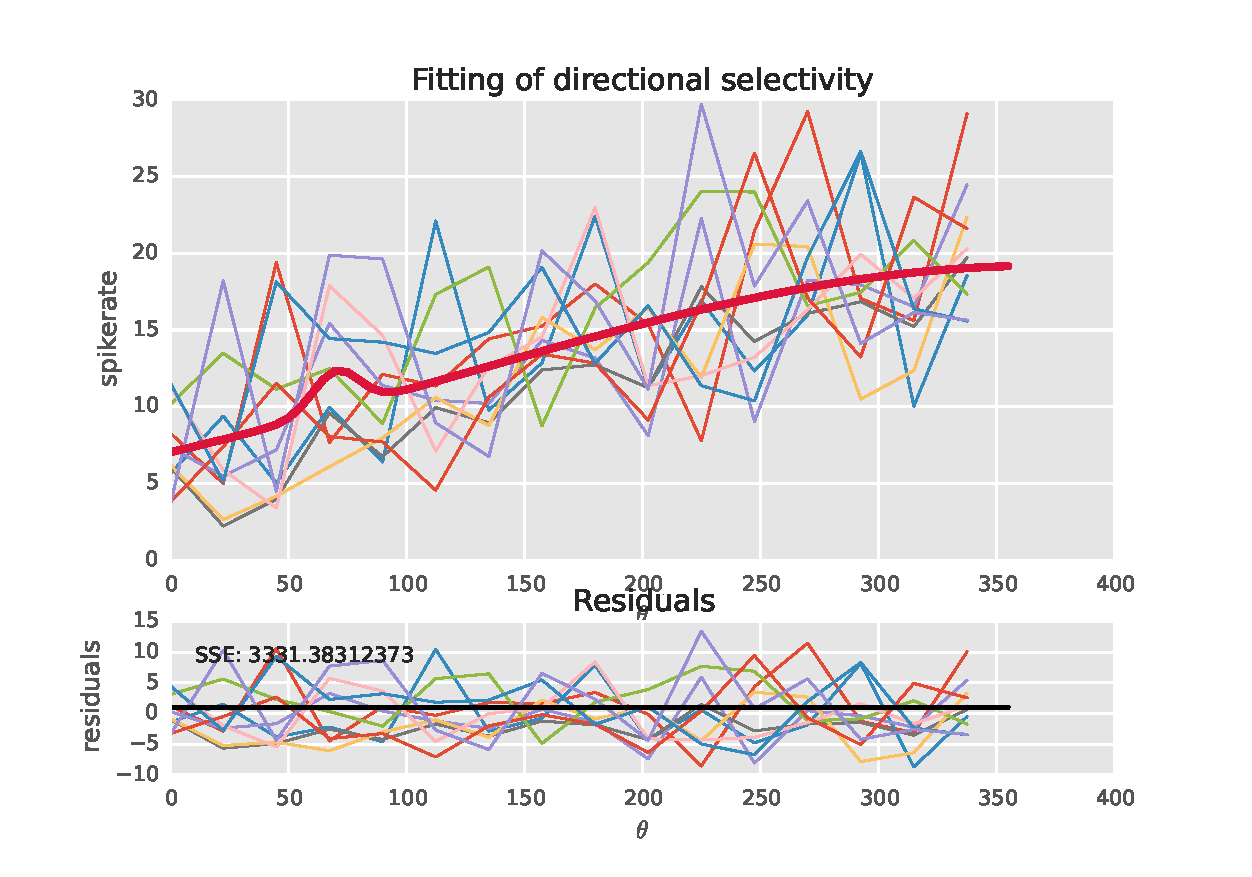
\includegraphics[width=\linewidth]{plots/fit_unsel4}
    \end{subfigure}
    \caption{Fit of directional selectivity of unselective. The red curves show the fit and other curves are measured data. Note the large residuals}
    \label{fit_unsel}
\end{figure}
% subparagraph results (end)


% subsubsection estimating_direction_fit (end)

% subsection modeling_the_neuron_response (end)
\FloatBarrier
\subsection{Classification of simple and complex cells} % (fold)
\label{sub:classification_of_simple_and_complex_cells}
The properties that distinguish the tree types of cells are discussed before. This problem statement deals with using machine learning tools for making a classifier for these three classes of cells.\\
The main challenge here is that we don not have the ground truth data for the data, which force us into category of unsupervised learning methods. This also makes it hard to evaluate the performance of the classification algorithm. We make an effort to classify cells based on some features extracted from the time series data. The feature selection process and the intuition behind it are discussed below.
\begin{itemize}
    \item OSI : This is a measure of orientation selectivity, as an individual feature this may not be a strong classifier as the measure is not very robust, but along with other features, this could contribute towards classification.
    \item DSI : This is a measure of directional selectivity, as an individual feature this may not be a strong classifier as the measure is not very robust, but along with other features, this could contribute towards classification.
    \item $L_{ori}$ : This is more robust than OSI, and is expected to be a better feature.
    \item $L_{dir}$ : This is more robust than DSI, and is expected to be a better feature.
\end{itemize}
Following unsupervised learning techniques are use for the classification.
\subsubsection{k-means clustering} % (fold)
\label{ssub:k_means_clustering}
We hope that three classes of cells will form three clusters in the feature space. We run the algorithm with 3 clusters and features selected above.\\
As we said,  analyzing efficiency of classification is hard without ground truth. Here, what we use to analyze is this:
\begin{itemize}
    \item Find the global mean
    \item Find the sum of squared distance of each point in feature space to global mean. denoted by $total\_ss$.
    \item Find the sum of squared distance of each centroids to the global mean multiplied by number points in the cluster. denoted by $between\_ss$.
    \item If there is no well clustering, the centroids will be close to the global mean, and $between\_ss$ will be small compared to $total\_ss$.
    \item If $clusterEfficiency = between\_ss/total\_ss$ is high, the clustering is good and forms distinct clusters.
\end{itemize}
Table~\ref{tab:cluster_efficiency} shows the clustering efficiency in each mice.
\begin{table}[ht]
    \centering
    \begin{tabular}{| l || c |}
        \hline
        Subject & Cluster efficiency (\%)\\
        \hline
        \hline
        Mouse A & 78.8155 \\
        \hline
        Mouse B & 72.3963 \\
        \hline
        Mouse C & 72.293 \\
        \hline
        Mouse D & 78.8882 \\
        \hline
        Mouse E & 76.4573 \\
        \hline
    \end{tabular}
    \caption{Cluster efficiency of various subjects}
    \label{tab:cluster_efficiency}
\end{table}
The clustering was done is a higher dimensional space and hard to visualize, In figure, we show clustered neurons in a subspace of original feature space.
\begin{figure}[h]
    \centering
    \label{clusters}
    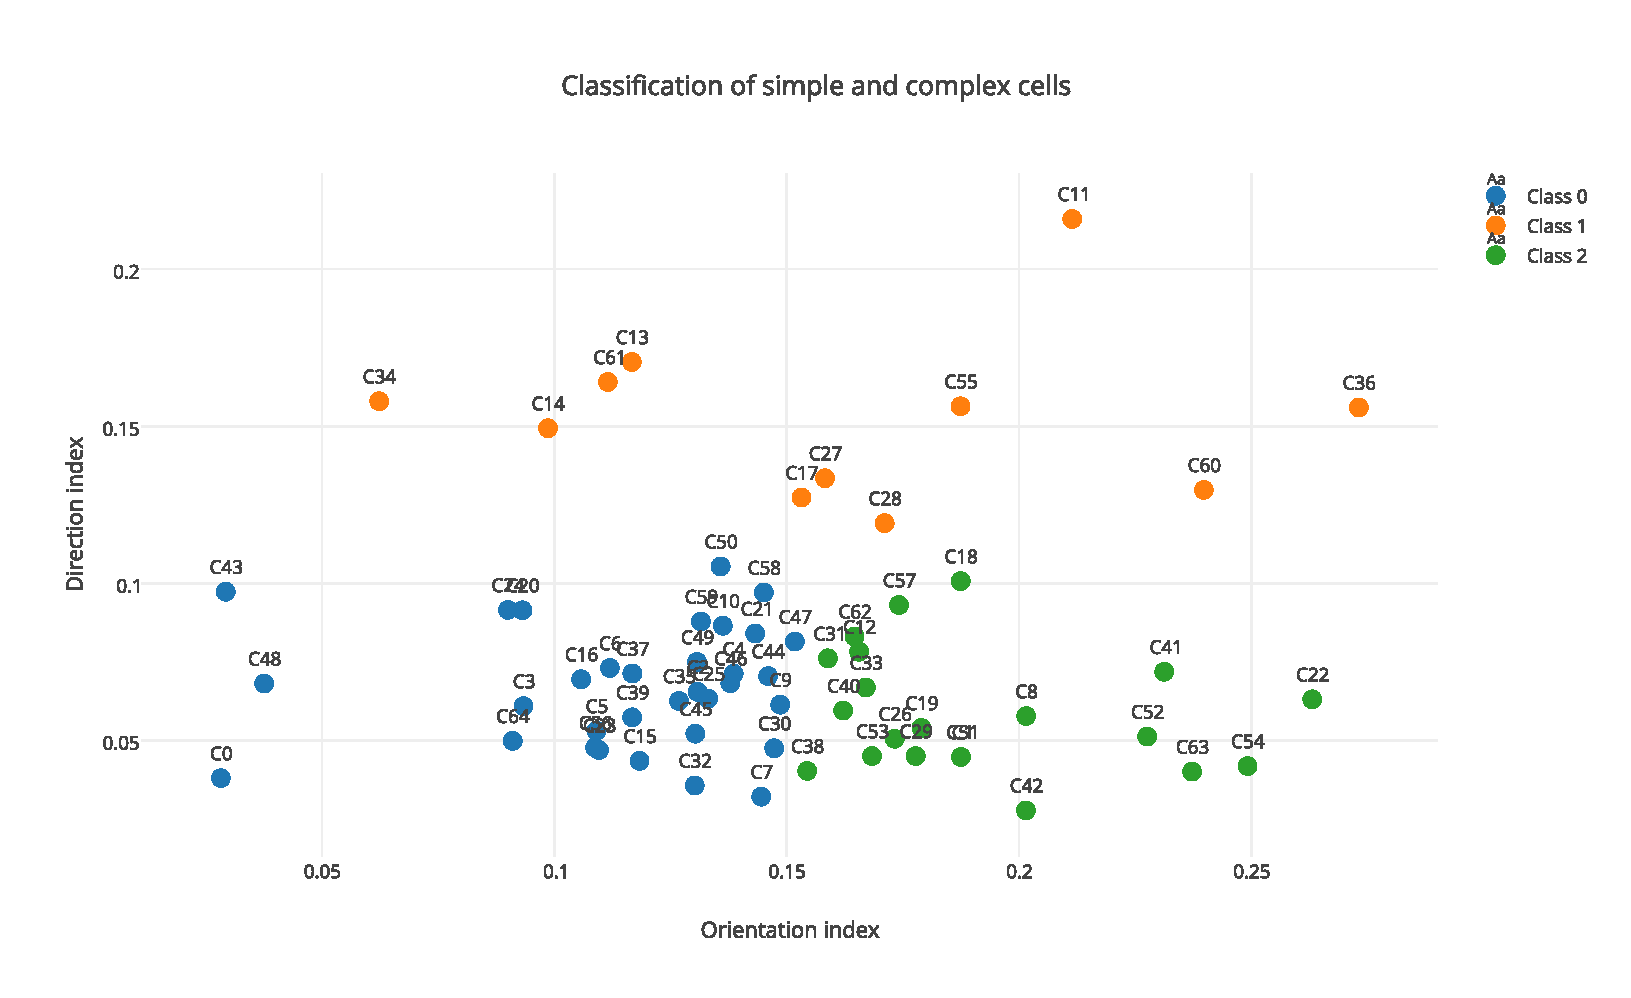
\includegraphics[width=.8\textwidth]{plots/clusters}
    \caption{Clustering result in a subspace of feature vector}
\end{figure}
% subsubsection k_means_clustering (end)
% subsection classification_of_simple_and_complex_cells (end)
\subsection{Study of correlation} % (fold)
\label{sub:study_of_correlation}
The activity of a population of cells was recorded. We would like to study the functional similarities of different neurons in a mouse. We aim to find out similarly tuned neurons. We could study the effects of receptive fields by this hopefully.\\
Similarly tuned cells are expected to have similar tuning curves (The double Gaussian we modeled before). We can study the pairwise correlation of tuning curves as first approach. Estimating correlation of the tuning curve may not be close to accurate as there are only 160 samples per neuron. The Figure~\ref{tuningCorr} shows heat map of correlations between tuning curves.
\begin{figure}[h]
    \centering
    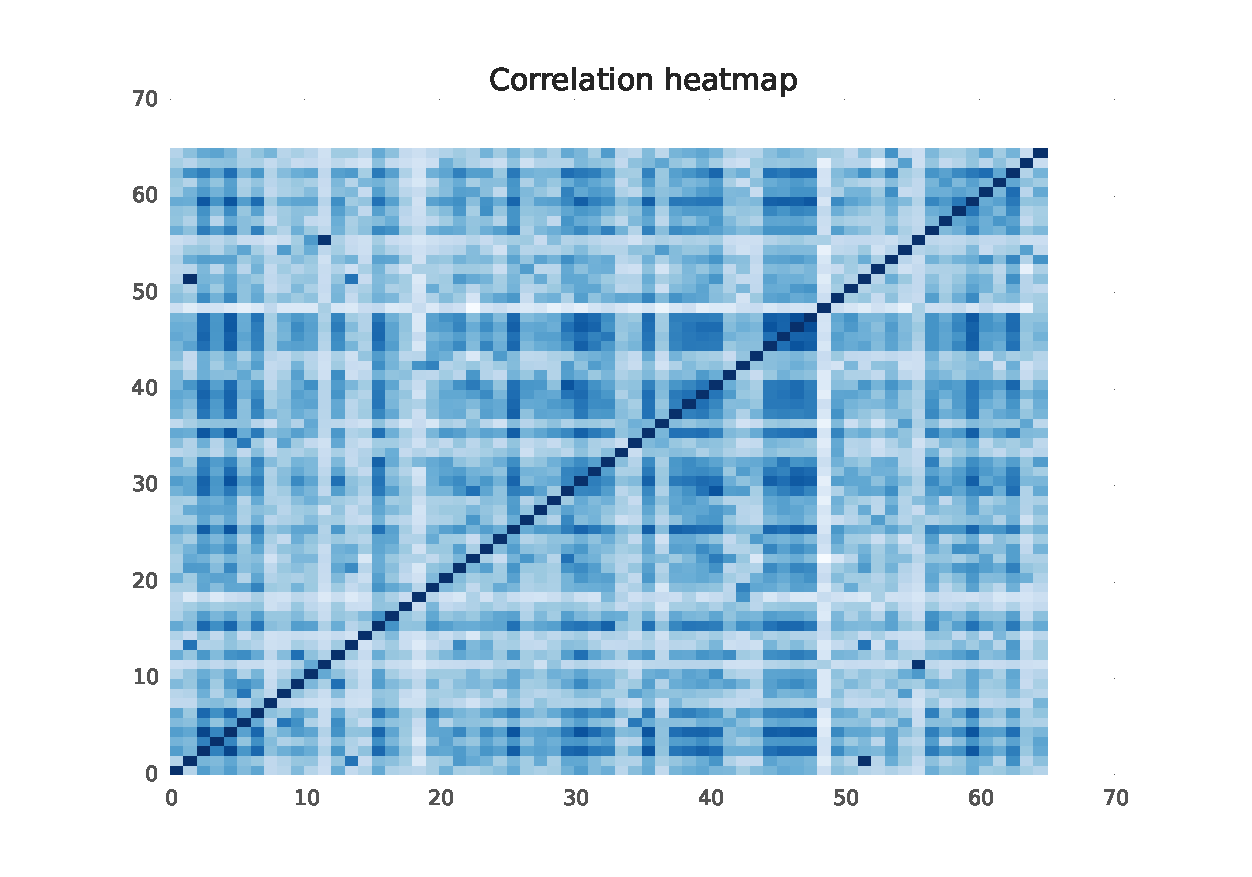
\includegraphics[width=\textwidth]{plots/tuningCorr}
    \caption{Heatmap of correlations between the tuning curves}
    \label{tuningCorr}
\end{figure}
To see the sanity of the results, we could plot tuning curves of neurons with high correlation.

% subsection study_of_correlation (end)
% ======================= References ==========================
\newpage
\bibliographystyle{plain}
% argument is your BibTeX string definitions and bibliography database(s)
% \bibliography{test}
\bibliography{../../bibliography/imgProc}
\end{document}